\begin{figure}
 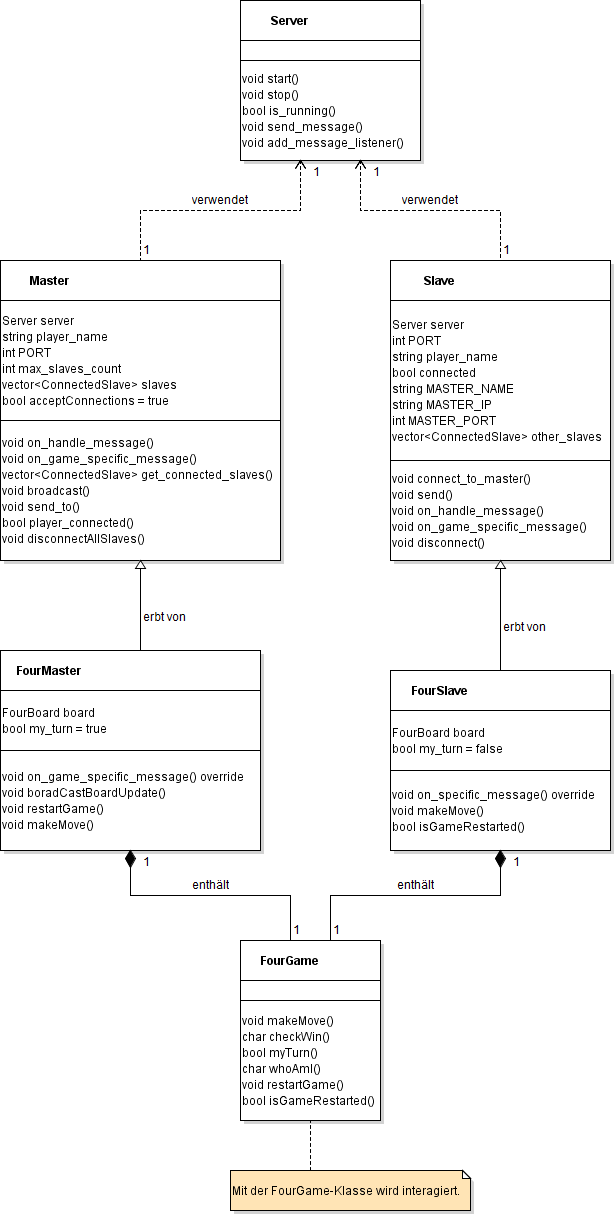
\includegraphics[height=\textheight]{UML/NetzwerkUML.png}
 \caption{Overview of the Network Part of the App}
\end{figure}
\subsection{Grundlegende Netzwerkfunktion}
Als erstes stellte sich die Frage, welche Art der Datenübertragung für TicTacToe und Vier gewinnt am sinnvollsten ist.
Ich musste mich hier zwischen UDP und TCP entscheiden. Beide haben Vor- und Nachteile, die für Echtzeitspiele zu beachten sind:
\par
Heutige Onlinespiele verwenden häufig UDP, da dieses Protokoll verbindungslos ist.
Das bedeutet bei einer Übertragung wird ein Paket ohne Absicherung verschickt. Der Sender kann dabei nicht wissen, ob das Paket
beim Empfänger angekommen ist oder, falls mehrere Pakete gesendet wurden, ob diese in der richtigen Reihenfolge beim Empfänger
eingetroffen sind.
Bei kurzen Statusmeldungen in Spielen, wie Positionsupdates von Spielern, ist UDP passend, da diese Updates sehr schnell wieder
durch neuere Informationen obsolet werden. Der Client sollte sich also nicht damit beschäftigen alte Pakete zu `retten`, sondern
möglichst immer bereit für das neuste Paket sein.
\par
Es gibt aber verschiedene Gründe TCP in Spielen zu verwenden.
Gerade wenn es sich bei den zu übertragenden Daten um wichtige Statusmeldungen handelt, die nur einmalig kommuniziert werden,
ist es wichtig, dass diese beim Empfänger ankommen. Wenn beispielsweise ein Spieler einem Spiel beitritt, wäre es fatal,
wenn diese Information bei einem der Mitspieler nicht ankommt. Die Spielumgebung wäre nicht mehr gleich für alle Teilnehmer
und das Spiel unter Umständen garnicht spielbar. TCP eignet sich sehr gut für solche Statusmeldungen, da es erst eine Verbindung aufbaut.
Solange diese Verbindung existiert, ist garantiert, dass die gesendeten Pakete eintreffen. Auch die richtige Reihenfolge ist garantiert.
\par
Wenn man sich Spiele wie TicTacToe und Vier gewinnt anschaut, bemerkt man schnell das diese Spiele keine großen Mengen von Updates
der Spielumgebung benötigen. Es sind nur wenige, dafür aber kritische Meldungen erforderlich, um die Spiele für beide Teilnehmer
synchron zu halten.
\par
Benötigt werden beispielsweise für TicTacToe:
\begin{itemize}
    \item Statusmeldung wo ein Spieler sein X oder O setzt.
    \item Statusmeldung ob jemand gewonnen hat und wer.
    \item Statusmeldung über den Abschluss des Spiels wenn das Spielbrett voll ist und es keinen Sieger gibt.
    \item Statusmeldung für den Neustart des Spiels.
\end{itemize}
Alle diese Meldungen sind per TCP besser umzusetzen, da sie in jedem Fall beim Empfänger ankommen müssen. Sonst wäre das Spiel
nicht mehr synchron und ggf. in einem undefinierten Zustand.
\subsection{Implementierung der Grundfunktionen}
Da wir uns für die Entwicklung für Android NDK entschieden haben, setzte ich die Implementierung in C++ um.
Dafür war es notwendig zu verstehen, wie C++ mit der normalerweise unter Android verwendeten Programmiersprache Java
zusammen arbeitet.
Das Java Native Interface (JNI) wird benutzt, um Objekte zwischen Java und C++ hin und her zu `senden`. Diese Übertragungen sind allerdings
zeitaufwendig. Da der visuelle Teil mit ARCore von David auch in C++ implementiert wurde, wollte ich das Netzwerk auch in C++ umsetzen.
\par
Zuerst habe ich Sockets verwendet, um Rohdaten empfangen und senden zu können.
In unseren Meetings mit Herrn Uhlmann wurde mir dann vorgeschlagen statt Rohdaten Structs zu verschicken.
Nachdem ich das umgesetzt hatte, wurde diese Idee in einem weiteren Meeting erweitert zu Message-Klassen, welche Methoden mitbringen,
mit denen die Objekte sich selbst in einen Bytestrom übersetzen und sich aus einem solchen Bytestrom wieder rekonstruieren können.
\subsection{Asynchrones Empfangen}
Als nächstes befasste ich mit dem asynchronen Empfangen der Daten. Da man dauerhaft mit einer Funktion auf eine TCP-Verbindung warten muss,
um dann die Nachricht zu verarbeiten, macht es Sinn, zumindest das Warten auf neue Verbindungen in einem seperaten Thread zu realisieren.
Dieser Thread ruft dann eine Callbackfunktion auf, die dann mit der Nachricht weiterarbeiten kann.
\subsection{Asynchrones Senden}
Das asynchrone Senden hatte ich mir erst im späteren Verlauf des Projektes vorgenommen. Ich dachte, dass das Senden nicht sonderlich
zeitaufwendig sein würde und den Spielfluss kaum beeinträchtigen könnte. Damit lag ich falsch. Wenn nämlich ein Fehler beim Senden
auftritt oder das Senden länger braucht als sonst, kann das die ganze App anhalten. Das ist natürlich nicht erstrebenswert.
Also realisierte ich eine Warteschlange in die Nachrichten eingefügt werden. Diese versendet dann der Reihe nach ein anderer Thread.
Bei einer langsamen Verbindung wird dann nicht die gesamte App verlangsamt.
\subsection{Abstraktion}
In Spielen gibt es im Netzwerk oft eine Hierarchie, welche regelt, wer der Host eines Spiels ist und wer nur als Client beitritt.
In unserem Projekt haben wir die Begriffe Master und Slave gewählt.
Der Master hält den einzig wahren Spielzustand. Die Slaves übernehmen diesen und senden dem Master ihre Spielzüge wenn
sie an der Reihe sind. Wenn der Master den Spielzug als valide einstuft, werden entsprechende Änderung
am Spielfeld vorgenommen und diese allen Slaves mitgeteilt.
So ändert ein Slave also nie sein eigenes Spielfeld. Nur der Master kann Änderungen für sich und alle Slaves durchführen.
Dadurch wird es viel einfacher die Spielfelder zwischen allen Spielern synchron zu halten.
\subsection{Konkrete Umsetzung für Spiele}
Um für David den Netzwerkcode einfach zugreifbar zu machen, habe ich Subklassen von Master und Slave für das jeweilige Spiel abgeleitet.
Diese können dann genutzt werden, um Spielzüge zu machen, ohne dass man sich um die Netzwerkschnittstelle kümmern muss.
Master und Slave sind dann nochmal in einem Game-Objekt zusamengefasst, damit David den Code für Master und Slave
einheitlich aufrufen kann.

\subsection{Testen der Netzwerkfunktionen}
Ursprünglich wollte ich den Emulator nutzen, um die Kommunikation zwischen zwei Instanzen der App zu testen.
Der Emulator hat allerdings eine eigene Firewall, welche für mich nicht so offensichtlich zu konfigurieren war.
Zusätzlich hatte ich das Problem, dass mein eigentlicher Arbeitscomputer durch unglückliche Umstände keine Virtualisierung unterstützt.
Dadurch musste ich für die Emulation immer einen seperaten PC verwenden. Das war mir auf Dauer dann zu aufwendig und so entschied ich mich
ein Python-Skript zu schreiben. Damit sollte man das TicTacToe-Spiel in der Kommandozeile gegen einen Spieler mit der App spielen können.
Das Skript kann die Rolle des Masters und des Slaves einnehmen. Damit gelang es dann auch die Netzwerkfunktionen zu testen.

\subsection{Aufbauen der Verbindung in der App}
Damit Spieler nicht IP-Adressen auslesen und eintippen müssen, erfolgt der Austausch über einen
QR-Code. Diese Idee kam David, als er beim Testen der App ständig seine IP-Adresse eingeben musste.
Der Spieler, der das Spiel als Master eröffnet, kann nun einfach einen QR-Code generieren
und anzeigen lassen, welcher die lokale IP-Adresse des Geräts enthält.
Der beitretende Spieler kann diesen in seiner App einscannen
und die Verbindung einfach und bequem aufbauen.
